The plugin stores data in a format which enables performing semantic analysis on the data. 
Instead of storing all objects in a single file, tt stores every HDF5 object in a separate location, so that data from different objects is not contained in the same file. 
The central object store in HDF5, the HDF5 file, is represented by a directory. Groups are stored as directories as well, whereas datasets, which contain raw data, are stored in files. 
The relationship between objects is explained by the relative paths between the objects at the file system level. Consider the example shown in figure~\ref{hdf5_example}. Using the plugin, file Sample.h5 is stored as a directory. Group G1 is stored as a directory under it, and datasets D1 and D2 are files. We can see that the relationship between the objects is represented by their relative paths at the file system as shown in figure~\ref{hdf5_example_plugin}. This way, the plugin eliminates the need to store the metadata describing the relationship between objects. Metadata about datasets, such as the datatype, extent, dimensions etc., are stored as PLFS Xattributes (xattrs) as explained in the previous section. 
\begin{figure}[!t]
\centering
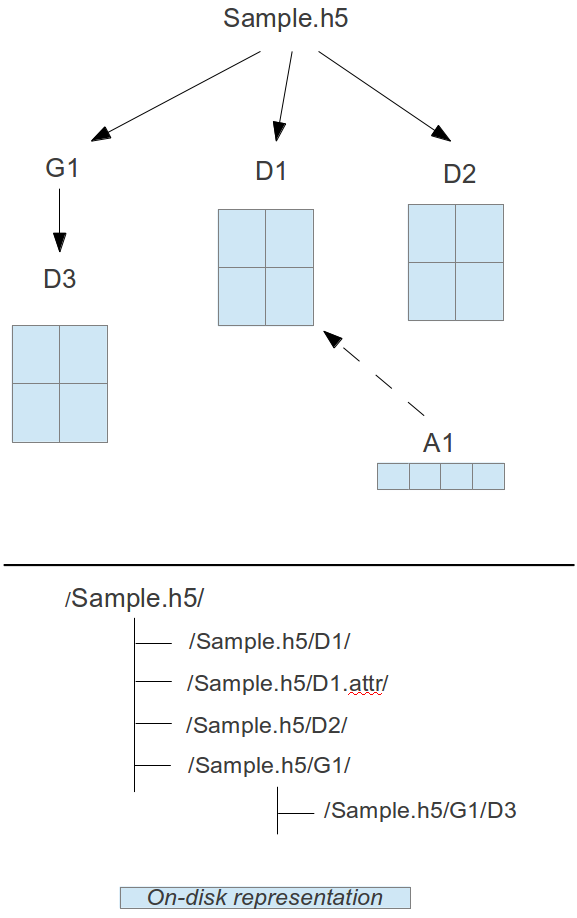
\includegraphics[width=2.5in]{hdf5_example_plugin}
\caption{HDF5 file created using our PLFS plugin}
\label{hdf5_example_plugin}
\end{figure}

This approach gives us the ability to distinguish HDF5 objects at the file system level, without requiring an HDF5 application to provide information about objects and the relationship between them. 
It enables us to perform post-processing and semantic analysis on the data, outside the scope of the HDF5 application. 

Implementing the plugin requires providing an implementation for a "driver" interface provided by HDF5. In short, we provide an implementation for all functions that access data on disk. This includes functions for file management, dataset creation and access, group creation, to name a few.

%The following table lists the VOL functions currently provided by the PLFS plugin:
%\begin{itemize}
%\item Attribute yes
%\item Dataset yes
%\item File yes
%\item Group yes
%\item Object No
%\item Link No
%\end{itemize}

